\section{Trust Region Policy Optimization (TRPO)}
\begin{frame}{}
    \LARGE Policy Optimization: \textbf{TRPO}
\end{frame}

\begin{frame}{TRPO: KL Trust Region}
\begin{itemize}
    \item TRPO formalises the constraint: maximize the surrogate objective subject to a KL-divergence bound:
    $$\max_\theta\; \mathcal{L}(\theta) \quad \text{s.t.} \quad \mathbb{E}_t\!\left[ D_{KL}\!\left(\pi_{\theta_\text{old}}(\cdot|s_t) \,\|\, \pi_\theta(\cdot|s_t)\right) \right] \leq \delta$$
    \item Keeps the new policy inside a \textbf{trust region} in policy space, not parameter space
    \item Solved with conjugate gradient + backtracking line search (second-order): largest natural-gradient step that still satisfies the KL constraint
    \item \textbf{Cost:} needs the Fisher information matrix --- expensive and hard to scale. \emph{This is exactly what motivates PPO.}
\end{itemize}
\end{frame}

\begin{frame}{TRPO: Trust Region in Policy Space}
\begin{center}
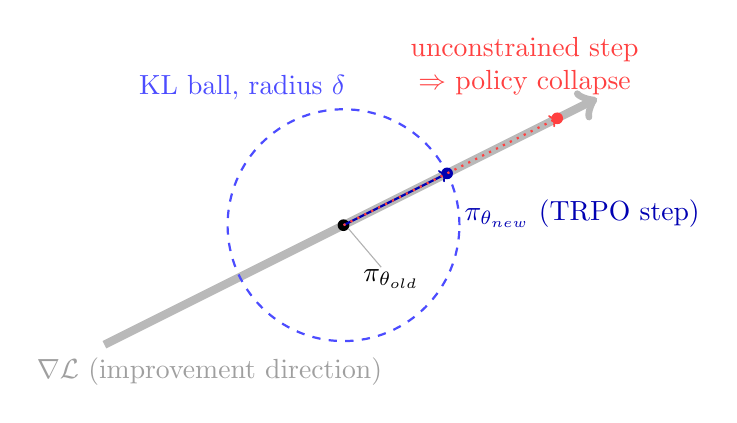
\begin{tikzpicture}[scale=0.92]
    % surrogate-objective improvement direction (background gradient hint)
    \draw[->, gray!55, line width=3pt] (-3.3,-1.65) -- (3.5,1.75);
    % gradient label: horizontal, parked in the clear lower-left wedge
    % (below the arrow band and outside the KL ball)
    \node[gray!75, anchor=north] at (-1.85,-1.7) {$\nabla \mathcal{L}$ (improvement direction)};

    % KL trust region: a ball around theta_old
    \draw[dashed, thick, blue!70] (0,0) circle (1.6);
    \node[blue!70] at (-1.4,1.9) {KL ball, radius $\delta$};

    % old policy --- label offset perpendicular to the arrow (lower-right clear zone)
    \fill (0,0) circle (2.3pt);
    \node[black] at (0.66,-0.74) {$\pi_{\theta_\text{old}}$};
    \draw[gray!60, line width=0.4pt] (0.07,-0.05) -- (0.52,-0.58);

    % constrained TRPO step: stops at the boundary
    \draw[->, thick, blue!70!black] (0,0) -- (1.43,0.715);
    \fill[blue!70!black] (1.43,0.715) circle (2.3pt);
    \node[blue!70!black, below right=1pt] at (1.5,0.52) {$\pi_{\theta_\text{new}}$ (TRPO step)};

    % unconstrained step: overshoots -> collapse
    \draw[->, thick, red!75, dotted] (0,0) -- (2.95,1.475);
    \fill[red!75] (2.95,1.475) circle (2.3pt);
    \node[red!75, align=center] at (2.5,2.2) {unconstrained step\\$\Rightarrow$ policy collapse};
\end{tikzpicture}
\end{center}
\begin{itemize}
    \item Each update stays within a \textbf{KL ball} around $\pi_{\theta_\text{old}}$ (\emph{policy} space, not parameter space): the step climbs $\mathcal{L}$ but is clipped at the boundary, preventing the overshoot that collapses the policy
\end{itemize}
\end{frame}
